\chapter{RESULTADOS}

Este capítulo reporta el estado experimental de CAVA al congelar el sistema (commit
\texttt{d51d201}, 25 pruebas automatizadas en verde). Los números provienen de corridas
completas guardadas en \texttt{results/} y del registro de experimentos EXP-009 a EXP-039.

\section{Experimentos y resultados}

\subsection{Pilotos del gestor sin fusión}

El mecanismo de consenso se verificó primero con datos sintéticos de dos señales y después en
video real. En 3 videos de TVSum, con transcripción, señal visual SigLIP/BaSSL y densidad de
voz, los grupos resultantes siguieron los pasos del contenido (por ejemplo, seguridad,
evaluación del clavo, inflado, solución de problemas y taller en un video sobre reparar un
neumático) y cada grupo tuvo soporte de varias señales. El piloto en BLiSS, con
transcripciones reales, mostró el primer problema de calibración: un embedding de texto
(RoBERTa) que se agrupa por locutor fragmenta el contenido en exceso (17 tópicos por clip), lo
que motivó los percentiles por perfil. En una validación paralela fuera de dominio, las
fronteras fueron estables en 4 dominios (AP de 0.73 a 0.78) y la correlación con la
importancia humana fue $\rho \approx 0$, lo que indica que una frontera temática y un momento
importante son cosas distintas.

\subsection{Mapa de tópicos en test (EXP-017 y EXP-018)}

EXP-017 encontró en desarrollo que el enlace por componentes conexas con retornos percola: sin
abstención, CAVA colapsa en unos 4 tópicos gigantes con una tasa de enlace de 0.99. EXP-018
pre-registró la corrección (abstención de las señales sin evidencia y enlace promedio) y la
evaluó en el split de test de 47 películas de MovieNet (Tabla~\ref{tab:exp018}).

\begin{table}[H]
    \centering
    \caption{Mapa de tópicos en test (47 películas, EXP-018). MCC por pares de unidades
    contra el proxy de reparto, número medio de tópicos por película y tasa de enlace.}
    \label{tab:exp018}
    \small
    \begin{tabular}{lccc}
        \hline
        \textbf{Sistema} & \textbf{MCC} & \textbf{N.$^{\circ}$ tópicos} & \textbf{Tasa de enlace} \\
        \hline
        \texttt{cava\_abst} (enlace promedio y abstención) & \textbf{0.0113} & 139.4 & 0.044 \\
        \texttt{cava\_abst\_r95} (percentil de retorno 95) & 0.0115 & 216.7 & 0.020 \\
        \texttt{cava} (componentes, sin abstención) & 0.0090 & 4.0 & 0.990 \\
        \texttt{cava\_avg} (enlace promedio, sin abstención) & 0.0083 & 90.7 & 0.054 \\
        visual sola & \underline{0.0195} & 56.6 & 0.248 \\
        VLM sola & 0.0079 & 32.4 & 0.159 \\
        \texttt{fused} (concatenación de señales) & 0.0053 & 39.7 & 0.197 \\
        diálogo sola & 0.0053 & 81.4 & 0.331 \\
        \texttt{contiguous} (gestor sin retornos) & 0.0045 & 86.0 & 0.001 \\
        \hline
    \end{tabular}
\end{table}

El criterio pre-registrado se cumplió: MCC(\texttt{cava\_abst}) $-$ MCC(\texttt{fused})
$= +0.0060 \pm 0.0024$ ($z = 2.46$), y frente al gestor contiguo la diferencia es $+0.0068
\pm 0.0027$ ($z = 2.48$). La Tabla~\ref{tab:ablacion} y la Figura~\ref{fig:ablacion}
separan las dos diferencias entre \texttt{cava\_abst} y \texttt{fused}. Sin abstención, no
fusionar las señales no basta para superar a la fusión: la diferencia es de $z = 0.80$ con
componentes conexas y de $z = 1.11$ con enlace promedio. La abstención agrega $+0.0030$
sobre el enlace promedio ($z = 1.78$), y solo la combinación de las dos cruza el umbral. Como
la abstención requiere que cada señal conserve su propia partición, la ganancia medida sí
depende de no fusionar, aunque por una vía indirecta.

\begin{table}[H]
    \centering
    \caption{Comparaciones pareadas en las 47 películas de test (EXP-018). Diferencia media de
    MCC por película $\pm$ error estándar. Solo la primera fila es el criterio
    pre-registrado; el resto es análisis secundario con el mismo script.}
    \label{tab:ablacion}
    \small
    \begin{tabular}{lcc}
        \hline
        \textbf{Comparación} & \textbf{Diferencia de MCC} & $z$ \\
        \hline
        \texttt{cava\_abst} $-$ \texttt{fused} (pre-registrada) & $+0.0060 \pm 0.0024$ & 2.46 \\
        \texttt{cava\_abst} $-$ \texttt{contiguous} & $+0.0068 \pm 0.0027$ & 2.48 \\
        \texttt{cava} $-$ \texttt{fused} & $+0.0037 \pm 0.0046$ & 0.80 \\
        \texttt{cava\_avg} $-$ \texttt{fused} & $+0.0031 \pm 0.0028$ & 1.11 \\
        \texttt{cava\_abst} $-$ \texttt{cava\_avg} & $+0.0030 \pm 0.0017$ & 1.78 \\
        \texttt{cava\_abst} $-$ visual sola & $-0.0082 \pm 0.0030$ & $-2.74$ \\
        \hline
    \end{tabular}
\end{table}

\begin{figure}[H]
\begin{center}
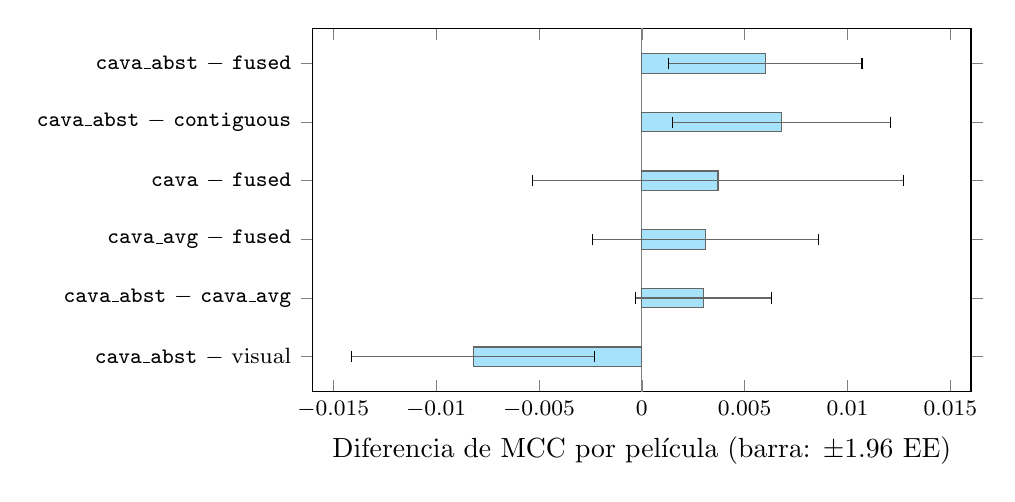
\begin{tikzpicture}
\begin{axis}[
  xbar, width=0.82\textwidth, height=6.2cm,
  xlabel={Diferencia de MCC por película (barra: $\pm 1.96$ EE)},
  symbolic y coords={absvis,abscava,avgfus,cavafus,abscont,absfus},
  ytick=data,
  yticklabels={\texttt{cava\_abst} $-$ visual, \texttt{cava\_abst} $-$ \texttt{cava\_avg},
               \texttt{cava\_avg} $-$ \texttt{fused}, \texttt{cava} $-$ \texttt{fused},
               \texttt{cava\_abst} $-$ \texttt{contiguous}, \texttt{cava\_abst} $-$ \texttt{fused}},
  yticklabel style={font=\footnotesize},
  xmin=-0.016, xmax=0.016,
  xtick={-0.015,-0.01,-0.005,0,0.005,0.01,0.015},
  xticklabel style={font=\footnotesize, /pgf/number format/fixed,
                     /pgf/number format/precision=3},
  scaled x ticks=false,
  bar width=7pt, enlarge y limits=0.12,
  extra x ticks={0}, extra x tick labels={},
  extra x tick style={grid=major, major grid style={black!50}},
]
\addplot[fill=cyan!35, draw=black!60,
  error bars/.cd, x dir=both, x explicit]
  coordinates {
    (-0.0082,absvis)  +- (0.0059,0)
    (0.0030,abscava)  +- (0.0033,0)
    (0.0031,avgfus)   +- (0.0055,0)
    (0.0037,cavafus)  +- (0.0090,0)
    (0.0068,abscont)  +- (0.0053,0)
    (0.0060,absfus)   +- (0.0047,0)
  };
\end{axis}
\end{tikzpicture}
\caption{Diferencias pareadas de MCC en el test de MovieNet (47 películas). Solo las
comparaciones de \texttt{cava\_abst} con \texttt{fused} y con \texttt{contiguous} quedan por
encima de cero; la señal visual sola supera a \texttt{cava\_abst}.}
\label{fig:ablacion}
\end{center}
\end{figure}

Los valores absolutos de MCC son bajos (alrededor de 0.01) porque el proxy de reparto mide
coaparición de personajes y no tópicos, y porque la tasa de pares positivos es alta. La señal
visual sola obtiene un MCC mayor que el consenso ($z = -2.74$ para la diferencia), lo que
indica que, en este proxy, las otras señales restan más de lo que aportan. En precisión de
enlace frente a la tasa base de pares positivos, \texttt{cava\_abst} supera a la base por
$+0.026$ ($z = 5.59$), la visual sola por $+0.016$ ($z = 4.31$) y \texttt{fused} por $+0.005$
($z = 1.95$). Lo que el consenso agrega sobre la señal visual sola es estructural: la
abstención elimina la percolación (de 4 a 139 tópicos y de 0.99 a 0.04 de tasa de enlace) y
cada grupo declara qué señales lo sostienen.

La compuerta G-coherencia se cumplió en las 47 películas: el margen intra$-$inter de
\texttt{cava\_abst} es positivo en todas para las tres señales, con medias de $+0.053$
(visual), $+0.018$ (diálogo) y $+0.121$ (VLM), frente a $+0.027$, $+0.007$ y $+0.067$ de la
fusión. El gestor contiguo tiene márgenes mayores ($+0.067$, $+0.049$ y $+0.155$), lo que es
esperable porque sus grupos están formados solo por unidades vecinas, que se parecen más
entre sí.

\subsection{Perfiles de contenido y ajuste de fronteras}

El perfil de documental se validó en BBC Planet Earth contra el acuerdo de 5 anotadores ($z =
6.1$ y $7.4$ en los dos criterios), con una estructura que alcanza el 62\,\% del acuerdo
humano. El ajuste de fronteras a cortes visuales certificados se validó en 91 películas ($z
= 26.6$ y $23.0$): las fronteras consensuadas caen en cortes reales sin desplazamiento
sistemático. En reuniones (AMI), el perfil de reunión iguala a la partición contigua
($+0.036 \pm 0.035$, $z = 1.0$) y los turnos de hablante como votante de fronteras aportan
$+0.075$ ($z = 2.32$). En este dominio la estructura temática es casi contigua, y el sistema
devuelve pocos enlaces no contiguos.

\subsection{Voz: votante, identidad y hablante único}

Como votante de tópico, la voz distingue pares de unidades con el mismo hablante con un AUC
de 0.72 a 0.74, frente a 0.55 de la señal visual (EXP-020a). La identidad de hablante
(WavLM-sv, Ward y BIC) supera a la agrupación por apariencia: ARI 0.186 frente a 0.038 en
desarrollo de AMI, con una especificidad de las identidades publicadas del 85\,\% (69 de 81,
$p \approx 0$, binomial). Con los filtros de habla entrenados, la identidad de voz llega a ARI
0.64 en VoxConverse y 0.73 en AMI (desde 0.25 y 0.29). El detector de hablante único no da
falsos positivos en 40 reuniones de AMI, pero tampoco detecta al narrador en ninguno de los
11 episodios de BBC; por eso el perfil de documental publica grupos acústicos y no personas.
La compuerta de AMI con el mapa completo resultó no inferior a la configuración base
($-0.007 \pm 0.009$, dentro del margen).

EXP-039 probó cinco detectores alternativos del hablante único sobre habla filtrada. En
desarrollo se eligió el de dispersión (\emph{spread}) con $\tau = 0.983$. En confirmación,
el detector no mejora la detección del hablante único frente al producto actual, ni con el
filtro S\&W ($-0.022 \pm 0.058$, $z = -0.37$) ni con I\&W ($0.000 \pm 0.062$, $z = 0.00$),
aunque cumple los criterios de falsos positivos (a lo sumo 0.019 en mezclas con varias voces
y ninguna reunión de AMI marcada). Según la lectura declarada en el pre-registro, ninguno de
los detectores probados conserva la detección del narrador, y el módulo queda como no
validado.

\subsection{Compuerta de versiones (G-versión)}

La verificación automática de presupuestos se cumplió en todos los conjuntos: 58 de 58
películas de MovieNet, 80 de 80 reuniones de AMI, 90 de 90 corridas del contrato v1 (los 40
videos web de VidChapters blind40 y los 50 de TVSum), 25 de 25 videos de SumMe y los 9 videos
del conjunto A/B. G-versión verifica existencia y presupuesto, no calidad percibida.

\subsection{Enlaces no contiguos (G-enlace)}

El primer lote de revisión con juez modelo dio 83\,\% frente a 63\,\% (Fisher $p = 0.072$),
con pocos casos y con revisores distintos en cada brazo. El segundo lote, pre-registrado con
el protocolo corregido (ciego, controles emparejados y 60 casos nuevos por brazo), dio 62\,\%
frente a 65\,\% ($p = 0.72$), de modo que G-enlace-2 no se cumple. La revisión de los casos
indica que los enlaces de CAVA capturan continuidad de personajes y situaciones, que el juez
reconoce, pero no la continuidad narrativa que exige un juez de trama. Por eso los retornos se
presentan como reagrupación temática con procedencia y no como tramas.

\subsection{Calidad automática de clips (EXP-031, EXP-037 y EXP-038)}

Ninguna regla de selección de clips superó a las bases simples con referencias automáticas.
En TVSum (EXP-031), los destacados de CAVA no difieren del azar ($+0.017 \pm 0.076$, $z =
0.22$) y quedan por debajo de un clip único en el centro del video ($-0.265 \pm 0.117$, $z =
-2.26$). Esa base aprovecha el sesgo de posición de los anotadores de TVSum, que puntúan más
alto la parte central del video. En SumMe (EXP-037), la mejor regla (H3, ventana saliente por
tópico) obtiene 0.278 frente a 0.156 de los clips equiespaciados, sin llegar a 2 errores
estándar ($z = 0.70$). La política de clips aprendida con un bandido contextual sobre TVSum
(EXP-038) obtiene en SumMe una recompensa de $-0.265$, peor que el azar ($z = -2.62$). TVSum
premia la mitad del video y SumMe el principio, y la política aprendió preferencias de
posición propias del conjunto de entrenamiento. En SumMe apareció además un defecto del
producto: en videos de menos de 50\,s, el 10\,\% de la duración no alcanza a cubrir una unidad
de 5\,s y los destacados salen vacíos. La corrección propuesta es exigir al menos una unidad.
Con estas referencias, la importancia humana de TVSum y SumMe y los capítulos de autor, no se
distingue a CAVA de las bases simples, porque cada referencia tiene su propio sesgo de
posición.

\subsection{Video web (EXP-032) y nivel de capítulo (EXP-033)}

Contra los capítulos de autor de VidChapters blind40, CAVA no supera a los cortes uniformes
con el mismo número de cortes ($-0.009$, $z = -0.44$) ni al mejor contiguo ($+0.046$, $z =
1.1$), y sí supera a la fusión en el tercer criterio pre-registrado ($+0.067 \pm 0.027$, $z =
2.46$). El nivel de tópico resulta unas 2.7 veces más fino que los capítulos de autor. El
nivel de capítulo por fronteras (las $N$ más fuertes) cumple el criterio de F1 de fronteras
($z = 2.57$) pero no el de agrupamiento ($z = 0.59$), por lo que queda como parcial y no se
incorpora al producto.

\subsection{Reconocimiento de voz (EXP-030)}

Se evaluó Parakeet TDT 0.6B v3 \cite{koluguri2024parakeet} como reemplazo de Whisper
large-v3. Empata en habla falsa ($+0.003$, $z = 0.11$), pierde menos en el número efectivo de
hablantes ($-0.039$) y es no inferior en MCC de AMI ($+0.015$, $z = 0.45$), pero omite seis
veces más habla (6.0\,\% frente a 1.5\,\%, fuera del margen de $+0.02$). Whisper large-v3 se
mantiene como transcriptor del producto.

\subsection{Evaluación con personas (EXP-040): estado}

El diseño compara, formato por formato, las versiones de CAVA con dos bases propias que
comparten unidades, corte, codificación, presupuesto y modelo de etiquetas: U, con clips
equiespaciados sin estructura, y S, con el mapa de la mejor señal sola (visual). Se propone
una tercera base, T: la segmentación que Claude Opus 5.5 produce leyendo solo los subtítulos
de YouTube, que permite medir si CAVA aporta algo sobre un modelo de lenguaje que solo usa el
texto. Cada participante ve dos versiones del mismo formato y video, en orden aleatorio y
sin saber su origen, elige una (o empate) y puntúa la utilidad de cada una. El resultado
principal por formato es la tasa de victoria de CAVA frente a U, con intervalos por bootstrap
sobre videos y participantes, y el ranking se estima con un modelo de Bradley--Terry
\cite{bradley1952rank}. Para detectar una preferencia de 60/40 con potencia 0.8 y $\alpha =
0.05$ se necesitan unos 200 juicios por formato, cerca de 1000 en total.

Al cierre de este documento, el conjunto de 9 videos está descargado y verificado, CAVA se
ejecutó sobre los 9 con el sistema congelado (G-versión 9/9, sin cambios locales en el
repositorio), la base T está generada para los 9 videos y la página de etiquetado ciego está
lista. Quedan pendientes el pre-registro, el etiquetado propio, el piloto y la evaluación
completa.

\subsection{Inventario del sistema}

La Tabla~\ref{tab:inventario} resume el estado de los 26 módulos del pipeline al congelarlo.
El detalle de cada fila, con la evidencia que la respalda, está en \texttt{docs/progress.md}.

\begin{table}[H]
    \centering
    \caption{Estado de validación de los 26 módulos de CAVA.}
    \label{tab:inventario}
    \begin{tabular}{p{2.6cm}cp{9.4cm}}
        \hline
        \textbf{Estado} & \textbf{N.$^{\circ}$} & \textbf{Módulos} \\
        \hline
        Validado & 10 & señal visual, voz como votante de tópico, gestor sin fusión, ajuste a
                         cortes visuales, perfiles de contenido, mapa con retornos y
                         procedencia, etiquetas de tópico, nombres de personajes, identidad de
                         voz, versiones con G-versión \\
        Acotado & 2 & VLM (sirve para enlazar, no como juez de trama); detector de hablante
                      único (no detecta al narrador) \\
        Parcial & 3 & turnos de hablante en reunión, filtro de habla, nivel de capítulo \\
        No validado & 6 & pesos de voto aprendidos, identidades por apariencia, regla de
                          destacados, regla H3, política de clips aprendida, detectores de
                          segunda voz (EXP-039) \\
        En producto sin compuerta propia & 4 & unidades fijas, transcripción, clips y
                          listas de reproducción, contrato de corrida \\
        Sin evaluación & 1 & exportación de datos de entrenamiento \\
        \hline
    \end{tabular}
\end{table}

Los módulos no validados quedan fuera del producto congelado, que usa pesos iguales, no
incluye el nivel de capítulo ni el filtro de habla, y selecciona destacados con la regla de
tópicos más largos.

\section{Discusión}

Los resultados apoyan la hipótesis estructural con una salvedad importante. El consenso con
abstención produce mapas de tópicos con mejor MCC que la fusión y que el gestor contiguo en
el test pre-registrado ($z = 2.46$ y $2.48$), y conserva márgenes de coherencia positivos en
todas las películas. Sin embargo, el efecto absoluto es pequeño, no fusionar las señales sin
abstención no basta para superar a la fusión, y la señal visual sola puntúa más alto en el
proxy disponible. El valor del sistema multimodal está en propiedades que el MCC no recoge:
la abstención evita la percolación (sin ella el mapa colapsa en 4 tópicos), cada grupo
declara qué señales lo sostienen, un mismo conjunto de perfiles cubre cuatro tipos de
contenido y del mismo mapa salen cinco formatos.

Las referencias automáticas de calidad de clips no distinguen a CAVA de bases simples, y una
política entrenada en un conjunto empeora en el otro. Esto no afecta al mapa, pero obliga a
medir la calidad de las versiones de otra forma: con preferencia humana directa, formato por
formato, frente a bases propias con el mismo presupuesto. Ese es el diseño de EXP-040, cuyo
conjunto de videos ya está procesado.

Hay cuatro amenazas a la validez. El proxy de reparto de MovieNet mide coaparición de
personajes y no trama, como también mostró G-enlace-2. La base \texttt{fused} es una
concatenación sin aprendizaje, más simple que la fusión con compuertas de A2Summ-X que motivó
el trabajo, de modo que la comparación no cubre las fusiones aprendidas. La evaluación en AMI
depende de que el corpus tenga disponible el video de cada reunión, y un trabajo de
extracción falló por archivos ausentes. Por último, los dominios sin anotación de tópicos
(YouTube largo, video de usuario) solo admiten referencias sustitutas, que este trabajo trata
como no concluyentes.
